% Metódy inžinierskej práce

\documentclass[10pt,twoside,slovak,a4paper]{article}

\usepackage[slovak]{babel}
\usepackage[IL2]{fontenc}
\usepackage{graphicx}
\usepackage{cite}
\usepackage{blindtext}
\usepackage[unicode]{hyperref}
\usepackage{capt-of}
\usepackage[document]{ragged2e}

\pagestyle{headings}

\title{\bf Elektronický poštový systém} 

\author{Mária Matušisková\\[2pt]
	{\small Slovenská technická univerzita v Bratislave}\\
	{\small Fakulta informatiky a informačných technológií}\\
	{\small Vedúci: Ing. Fedor Lehocki}
	}

\date{\small 18.október 2021}

\begin{document}
\maketitle

\pagenumbering{arabic}

\begin{abstract}
\begin{flushleft}
{\bf \hspace{0.1cm}E-mail môžeme považovať za predchodcu internetu a hral významnú rolu pri jeho vzniku. Dnes je používanie e-mailov bežná súčasť nášho života, tak ako je dôležité mať telefónne číslo, rovnako je podstatné mať aj e-mailovú adresu.\par
\vspace{0.15cm}
\hspace{0.6cm}V tomto dokumente sa zaoberáme vznikom prvej elektronickej pošty. Ako fungovala na jej počiatkoch a dnes. Povieme si o štruktúre mailového systému a jeho protokoloch ako SMTP, IMAP či POP. Zásadným bodom projektu je objasnenie algoritmu odosielania elektronickej pošty, čo všetko sa odohráva za jediným kliknutím „odoslať“. Následne si priblížime bezpečnosť a filtrovanie spamov,  ako mailové servery chránia používateľov pred malwermi a vírusmi.}\par
\vspace{.3cm}
\textbf{\textit{Kľúčové slová: e-mail; e-mailový server; algoritmus e-mailu}}
\end{flushleft}
\end{abstract}

\section{Úvod}
\hspace{0.5cm}E-mail je elektrické odosielanie a prijímanie správ medzi dvoma alebo viacerými adresátmi. Táto komunikácia by však nemohla fungovať bez protokolov ako IMAP, POP, SMTP. Ich úlohou je odoslať správu na druhý server, teda prijímateľovi správy. Adresát si tak vie správu otvoriť, prečítať a uložiť.\par
\vspace{-0.8cm}
\hbadness=1371
\hspace{0.5cm}\paragraph{Udržateľnosť a etika.}Pri zadávaní správy je dôležitý aj formát textu. Ako prvú informáciu zadávame komu chceme odkaz odoslať, ktorej e-mailovej adrese. Následne napíšeme predmet obsahu správy, o čom daná informácie bude. A nakoniec vypíšeme takzvané telo (body) správy, kde už je samotný obsah, môže sa tam nachádzať text alebo príloha. Tento formát sa nazýva MIME (viacúčelové rozšírenie internetovej pošty).\par
\vspace{0.15cm}
\hspace{0.5cm}S rozvojom e-mailov sa vyvinulo aj ich zabezpečenie. V niektorých prichádzajúcich mailoch sa vyskytujú vírusy, ktoré sa môžu rozšíriť aj do zariadenia adresáta. Osoba, ktorá tieto správy odosiela sa označuje ako spammer a nevyžiadaná pošta sa označuje ako SPAM. Na vyvarovanie sa pred týmito správami vznikol systém, ktorý filtruje a šifruje informácie na zvýšenie bezpečnosti pre používateľov.
\vspace{-0.2cm}
\paragraph{Spoločenské súvislosti.}Ochrániť sa pred škodlivými informáciami môžu aj samotní užívatelia a to informačnou a digitálnou gramotnosťou. V dnešnej dobe je nevyhnutná, pretože uchováva a reprezentuje mnoho informácii v technickej forme. Spoločnosť vyžaduje poznatky s ich správnym narábaním.  \\
\vspace{0.2cm}
\hspace{0.5cm}Záleží aj od e-mailovej domény, ktorú adresát používa. V tomto článku si povieme aj o najpoužívanejších z nich. par
Dôležité súvislosti sú uvedené v kapitolách 3 a 4.\par
\vspace{0.15cm}
\hspace{1cm}Záverečné poznámky prináša časť~\ref{zaver}.

\section{Vznik e-mailu} 

Za vznikom e-mailu stojí spoločnosť ARPANET. Táto organizácia bola sieť, ktorá spájala rad počítačov po celom oddelení a bola vytvorená agentúrou DARPA (Defense Advanced Research Agency), ktorá patrila pod ministerstvo obrany USA. Účelom zriadenia výskumnej organizácie ARPANET bolo udržanie technologického pokroku oproti súperiacemu Rusku, hlavne po úspešnej misii Sputnik.\\
\hspace{0.5cm}
Historicky prvý e-mail sa poslal 29.októbra 1969 o pol jedenástej večer a to práve sieťou ARPANET. Správa bola odoslaná študentom programovania menom Charlye Kline z počítača, ktorý patril Leonardovy Kleinrockému do počítača Stanfordského výskumného ústavu. 

\begin{figure*}[tbh]
\centering
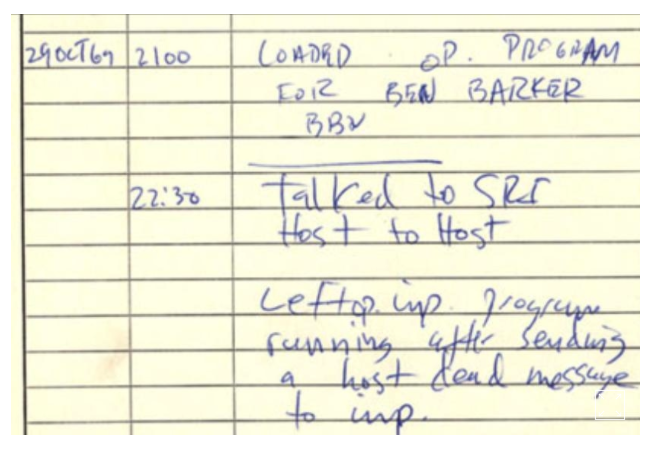
\includegraphics[scale=0.20]{firstmessage.png}
\caption{Prvá odoslaná elektronická správa \cite{UPI}}
\end{figure*}

Reálnu podobu systému odosielanie e-mailov akú poznáme dnes však vynašiel \textbf{Ray Tomlinson} v roku 1971. Dostal nápad skombinovať správu so systémom CPYNET (program určený na odosielanie súborov do druhého PC) cez sieť ARPANET:
\par
\vspace{.3cm}
\textit{,,V CPYNET proces používania prechádza cez Initial Connection Protocol (ICP) do servera socketu 7, čím sa vytvorí plne duplexné pripojenie s veľkosťou 8 bitov. Riadiace informácie vrátane používateľského mena, hesla, príkazu (čítanie, zápis alebo pridanie), názvu súboru a veľkosti bajtu pre dátové pripojenie sa prenášajú z procesu používania do procesu poskytovania. Pôvodné plne duplexné pripojenie sa potom uzavrie a vytvorí sa nové plne duplexné pripojenie s použitím pôvodných čísel socketu, ale s možnou inou veľkosťou bajtu. Súbor sa teraz prenáša na toto novo vytvorené spojenie. Koniec súboru je indikovaný zatvorením spojenia.} \cite{Bhushan}“
\par
\vspace{.3cm}
Vymyslel tiež systém pre identifikáciu adresy druhého počítača, kde sa meno používateľa oddeľuje od počítačového serveru za pomoci symbolu @ (at): ,,použivateľskémeno@menopočítača“.\\  
\hspace{0.5cm}
Bol to taký úspech, že do roku 1976 sa v organizácii ARPANET využíval tento systém na 75\% prevádzky. Postupom času sa začala riešiť nová problematika e-mailu. Spoločnosť chcela, aby sa elektronická pošta dala odoslať aj mimo internej siete a práve táto požiadavka motivovala myšlienku vzniku internetu. \\
\vspace{-0.3cm}
\paragraph{Historické súvislosti.}Na verejnej konferencii ICCC (International Computer Communication Conference) v roku 1972 ARPANET prvýkrát verejne predviedol túto myšlienku spolu s novinkou e-mailu. Už v roku 1973 sa internet stal medzinárodným spojením a to medzi USA a Spojením Kráľovstvom. Úplnej verejnosti sa odprezentoval v roku 1983.\\ 
\hspace{0.5cm}
Elektrická pošta sa rozšírila internacionálne v počiatkoch Internetu 80.rokov. Poskytovatelia internetových služieb začali vytvárať e-mailové hostingové stránky pre spájanie ľudí na celom svete. 
 
\hspace{0.5cm}V roku 1993 bola vynájdená bezdrôtová sieť (Wi-fi) čo túto službu ešte viac rozšírilo a do popredia sa dostali e-mailové servery ako AmericaOnline (AOL), EchoMail, Hotmail a Yahoo.\cite{UPI, Phrasee, Kleinrock}

\section{E-mailový systém} 

Na fungovanie e-mailu potrebujeme aplikačné softvéry na prijímanie, ukladanie a odosielanie správ. Takzvanú elektronickú schránku – mailbox. Poznáme súkromné (lokálne)  a webové servery. 

\begin{itemize}
\item súkromné servery
   \begin{itemize}
	\item Aplikácia je nainštalovaná v počítači a e-maily sú uložené priamo v zariadení. Nevýhodou je, že prístup k správam je obmedzený, nedá sa pripojiť k serveru z iného zariadenia, ktoré nie je prihlásené na túto aplikáciu. Dáta sa ukladajú do PC a nie na web. Využíva sa hlavne vo firmách a v podnikoch. Príkladom môžu byť aplikácie Microsoft Outlook, Thunderbird a ProtonMail. 
	\end{itemize}
\item webové servery
	\begin{itemize}
	\item Používateľ má prístup k mailovej schránke z rôzneho zariadenia, pretože server je na webovej adrese. Dáta sa ukladajú na web, je však menej bezpečnejší ako súkromný server. Príkladom sú služby ako Gmail, Yahoo a Webmail.
	\end{itemize}
\end{itemize}

\noindent{E-mailový systém funguje na vzájomnom prepojený protokolov a služieb.}\cite{GORALSKI}

\subsection{Služby} 

\textbf{UA (User Agent) /používateľská služba -} Adresát 1 vytvorí správu a odošle ju Adresátovi 2. Úlohou UA je vytvorenie a uloženie správy do mailovej schránky používateľa. U Adresáta 1 sa správa uloží ako odoslaná respektíve vytvorená a u Adresáta 2 sa správa uloží ako doručená.\cite{GORALSKI}\par
\vspace{0.4cm}
\textbf{MTA (The Message Transfer Agent)/služba prenosu súborov –} Nie vždy platí pravidlo, že druhý Adresát ma rovnaký mailový server. Úlohou MTA je spracovávanie spojenia medzi dvoma Adresátmi.\par Napríklad: \textit{menopouzivatela@\underline{gmail.com}}$\rightarrow$ \textit{menopouzivatela@\underline{yahoo.com}}\par
\vspace{0.4cm}
\textbf{MAA (Message Access Agent)/služba prístupu k správam –} Adresáti nie sú vždy prítomní na serveroch súčasne. Táto služba zabezpečuje načítanie e-mailu adresátom v danom čase, keď sa nachádzajú na servery alebo keď sú pripojení na sieti.\cite{GORALSKI}

\subsection{Protokoly} 

Na doručovanie e-mailov používame protokoly a každý protokol má náležitú funkciu. Najpoužívanejšie sú SMTP, POP, IMAP, ktoré patria pod TCP/IP (Transmission Control Protocol/Internet Protocol).\cite{GORALSKI}

\subsubsection{SMTP (Simple Mail Transfer Protocol)}

Je jednoduchý protokol na prenos elektronickej pošty cez internet. Pre lepšie pochopenie ho môžeme vnímať ako jazyk e-mailových serverov. Jeho hlavnou funkciou je zabezpečenie správy. Aby sa odkaz \textbf{doručil} určenému používateľovi a aby mal adresát istotu, že daný odkaz prijal od tej istej osoby. Overuje adresy domén používateľov a snaží sa tak zabrániť zneužitiu e-mailov. Ďalšou funkcie je šifrovanie správy, aby sa správa neodoslala len ako bežný čitateľný text. \\
\hspace{0.5cm}
Funguje ako priebeh odosielateľa/príjemcu, kde odosielateľ odošle príkazy (správu) a server ich vykoná, vráti kód odpovede (stavu) v prípade potreby. Ak prijímateľ akceptuje prichádzajúcu správu stáva sa odosielateľom SMTP.\cite{GORALSKI,active}

\subsubsection{POP (Post Office Protocol)}
\begin{sloppypar}
Aktuálnym protokolom je POP3, je určený hlavne pre občasných používateľov e-mailu. Jeho hlavnou funkciou je overenie správnosti správy a následne vymazanie (ak nespĺňa protokol) alebo zobrazenie správy prijímateľovi.\par
\end{sloppypar}
\hspace{0.5cm}
Prijímateľ musí e-mail stiahnuť zo servera do zariadenia, najprv sa stiahne až potom otvorí. Dôsledkom môže byť zachytenie vírusu či malvéru. Odoslané alebo vymazané správy sa stiahnuť nedajú a nie je možná organizácia súborov na servery. Nevýhodou tiež je, že automaticky po stiahnutí sa e-mail vymaže zo servera a už k nemu používateľ viac nemá prístup na opätovné stiahnutie. Výhodou ale je, že adresát má prístup ku e-mailom aj offline a šetrí internetový priestor.\cite{GORALSKI,pakistan}
\raggedbottom
\subsubsection{IMAP (Internet Message Access Protocol)}

Používateľ má prístup k elektronickej pošte cez internet vo forme webového prehliadača. E-mail môže otvoriť na viacerých zariadeniach súčasne bez toho, aby ich musel sťahovať. Možnosť triedenia a organizácie mailov do priečinkov. Spotrebuje viac CPU a pamäti než POP3, pretože ukladá dáta do vyrovnávacej pamäte. Najaktuálnejší protokol je IMAP4 a je zložitejší a drahší ako POP3.\cite{pakistan}

\section{Algoritmus e-mailu}
\begin{minipage}[tbh]{.49\textwidth}
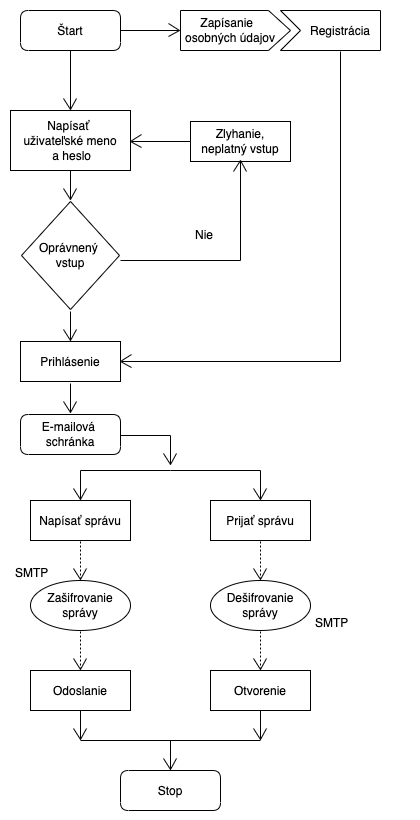
\includegraphics[width=0.8\linewidth]{algoritmus.png}
\captionof{figure}{Vývojový diagram \cite{Acharya_smartmailing}}
\end{minipage}
\begin{minipage}[thb]{.49\textwidth}
\begin{flushleft}
Do e-mailovej schránky sa dostaneme štandardným vstupom a to overením ID pošty používateľa.\par
\vspace{.2cm}
Používateľ si založí účet na e-mailovom servery. Základom je zápisanie osobných údajov používateľa a následná registrácia. Softvér tak overuje ID používateľa a zvyšuje bezpečnosť dôveryhodnosti.\par
\vspace{.2cm}
Ak je používateľ už zaregistrovaný, môže sa opakovane prihlasovať do jeho osobnej e-mailovej schránky. Pri každom prihlasovaný systém kontroluje ID používateľa cez vstup. Ak je zadané heslo nesprávne, program si vypýta zadanie údajov znova. 
Po prihlásení je užívateľ prenesený do prideleného e-mailového prostredia. \par
\vspace{.2cm}
Pri napísaní a posielaní správy, systém najprv správu zašifruje, aby sa tak zvýšila bezpečnosť. Zašifrovaná správa sa odošle určeným adresátom a po doručení sa automaticky dešifruje.\cite{Acharya_smartmailing}
\end{flushleft}
\end{minipage}

\section{Zabezpečenie a filtrácia spamov} 
\begin{flushleft}
S príchodom e-mailu sa začali vyskytovať v schránkach používateľov aj nežiadúce správy, takzvané spamy. Každým rokom ich objem narastá enormnou rýchlosťou, najčastejšie sa vyskytujúce typy sú ohľadom zdravia, zoznamky a finančných podvodov. Proti ich šíreniu a na zredukovanie množstva sa vyvíjajú rôzne filtračné techniky.\cite{heliyon}\\
\vspace{0.4cm}
\textbf{Technika filtrovaia podľa obsahu}\\
\vspace{0.1cm}
Filtruje e-maily podľa rôznych techník strojového učenia, príkladom je neuronová sieť. Táto technika má nastavené automatické pravidlá a vytvára si aj nové podľa určitých spôsobov a podmienok. Podľa týchto pravidiel analyzuje slová a frázy a následne filtruje. \\
\vspace{0.4cm}
\textbf{Heuristická technika filtrovania spamu}\\
\vspace{0.1cm}
Používa už vytvorené pravidlá alebo približné posudenie veľkého množstva vzorov, ktoré sú najčastejšími výrazmi voči vybranej správe. Vytvorí skoré podobnosti a pravdepodobnosti s porovnanými vzormi. Ak skóre prekročí zadanú hranicu, správa sa odfiltruje ako spam. 

\subsection{Najpoužívanejšie e-mailové servery} 
V súčastnosti najúspešnejšie zvládajú hrozbu spamov poskytovatelia ako Gmail, Yahoo a Outlook. Gmail dokáže odhaliť a odfiltrovať spam a phisingové e-maily s 99,9\% presnosťou. Považuje sa za najbezpečnejčí a najpouživanejší e-mailový server tejto doby. \cite{heliyon}


\section{Záver} \label{zaver} % prípadne iný variant názvu

V práci sme sa všeobecne zaoberali funkčnosťou e-mailu. Ozrejmili sme jeho počiatky až po súčastnosť. Definovali sme funkcie služieb a protokolov, ktoré na seba navzájom nadväzujú. Zaoberali sme sa aj problematikou spamov a aké najpoužívanejšie techniky ich filtrovania existujú. \\
\vspace{-0.2cm}
\paragraph{Technológia a ľudia.}Aj napriek pokročilosti doby e-mail stále patrí ku prvenstvu v komunikácii a je zaužívaný v spoločnosti. Najviac je však využívaný na formálne, edukačné a pracovné príležitosti.  
\end{flushleft}
%\acknowledgement{Ak niekomu chcete poďakovať\ldots}

\bibliography{literatura}
\bibliographystyle{abbrv}
\end{document}
